\centerline{\bf \Huge Геометрия 1. Точка Микеля}
\centerline{\bf \Huge Решения}

\begin{flushright}
        \scriptsize{}
\end{flushright}

\problem{1}
Четыре прямые $a, b, c$ и $d$ общего положения высекают на плоскости выпуклый четырехугольник $A B C D$.

(a) Докажите, что противоположные стороны этого четырехугольника видны из точки Микеля $M$ этой четверки прямых под равными углами.

\textbf{Решение.}
Точки $A, B, M, F$ коцикличны поэтому $\angle (AM, MB) = \angle (AF, FB)$. Аналогично для четверки $D, M, C, F$ имеет место равенство $\angle (DM, MC) = \angle (DF, DC)$. Но $\angle (DF, DC) = \angle (AF, FB)$, так как тройки точек $A, D, F$ и $F, C, B$ коллинеарны. Стало быть $\angle(AM, MB) = \angle(DM,MC)$, а это и означает требуемое.

\begin{center}
    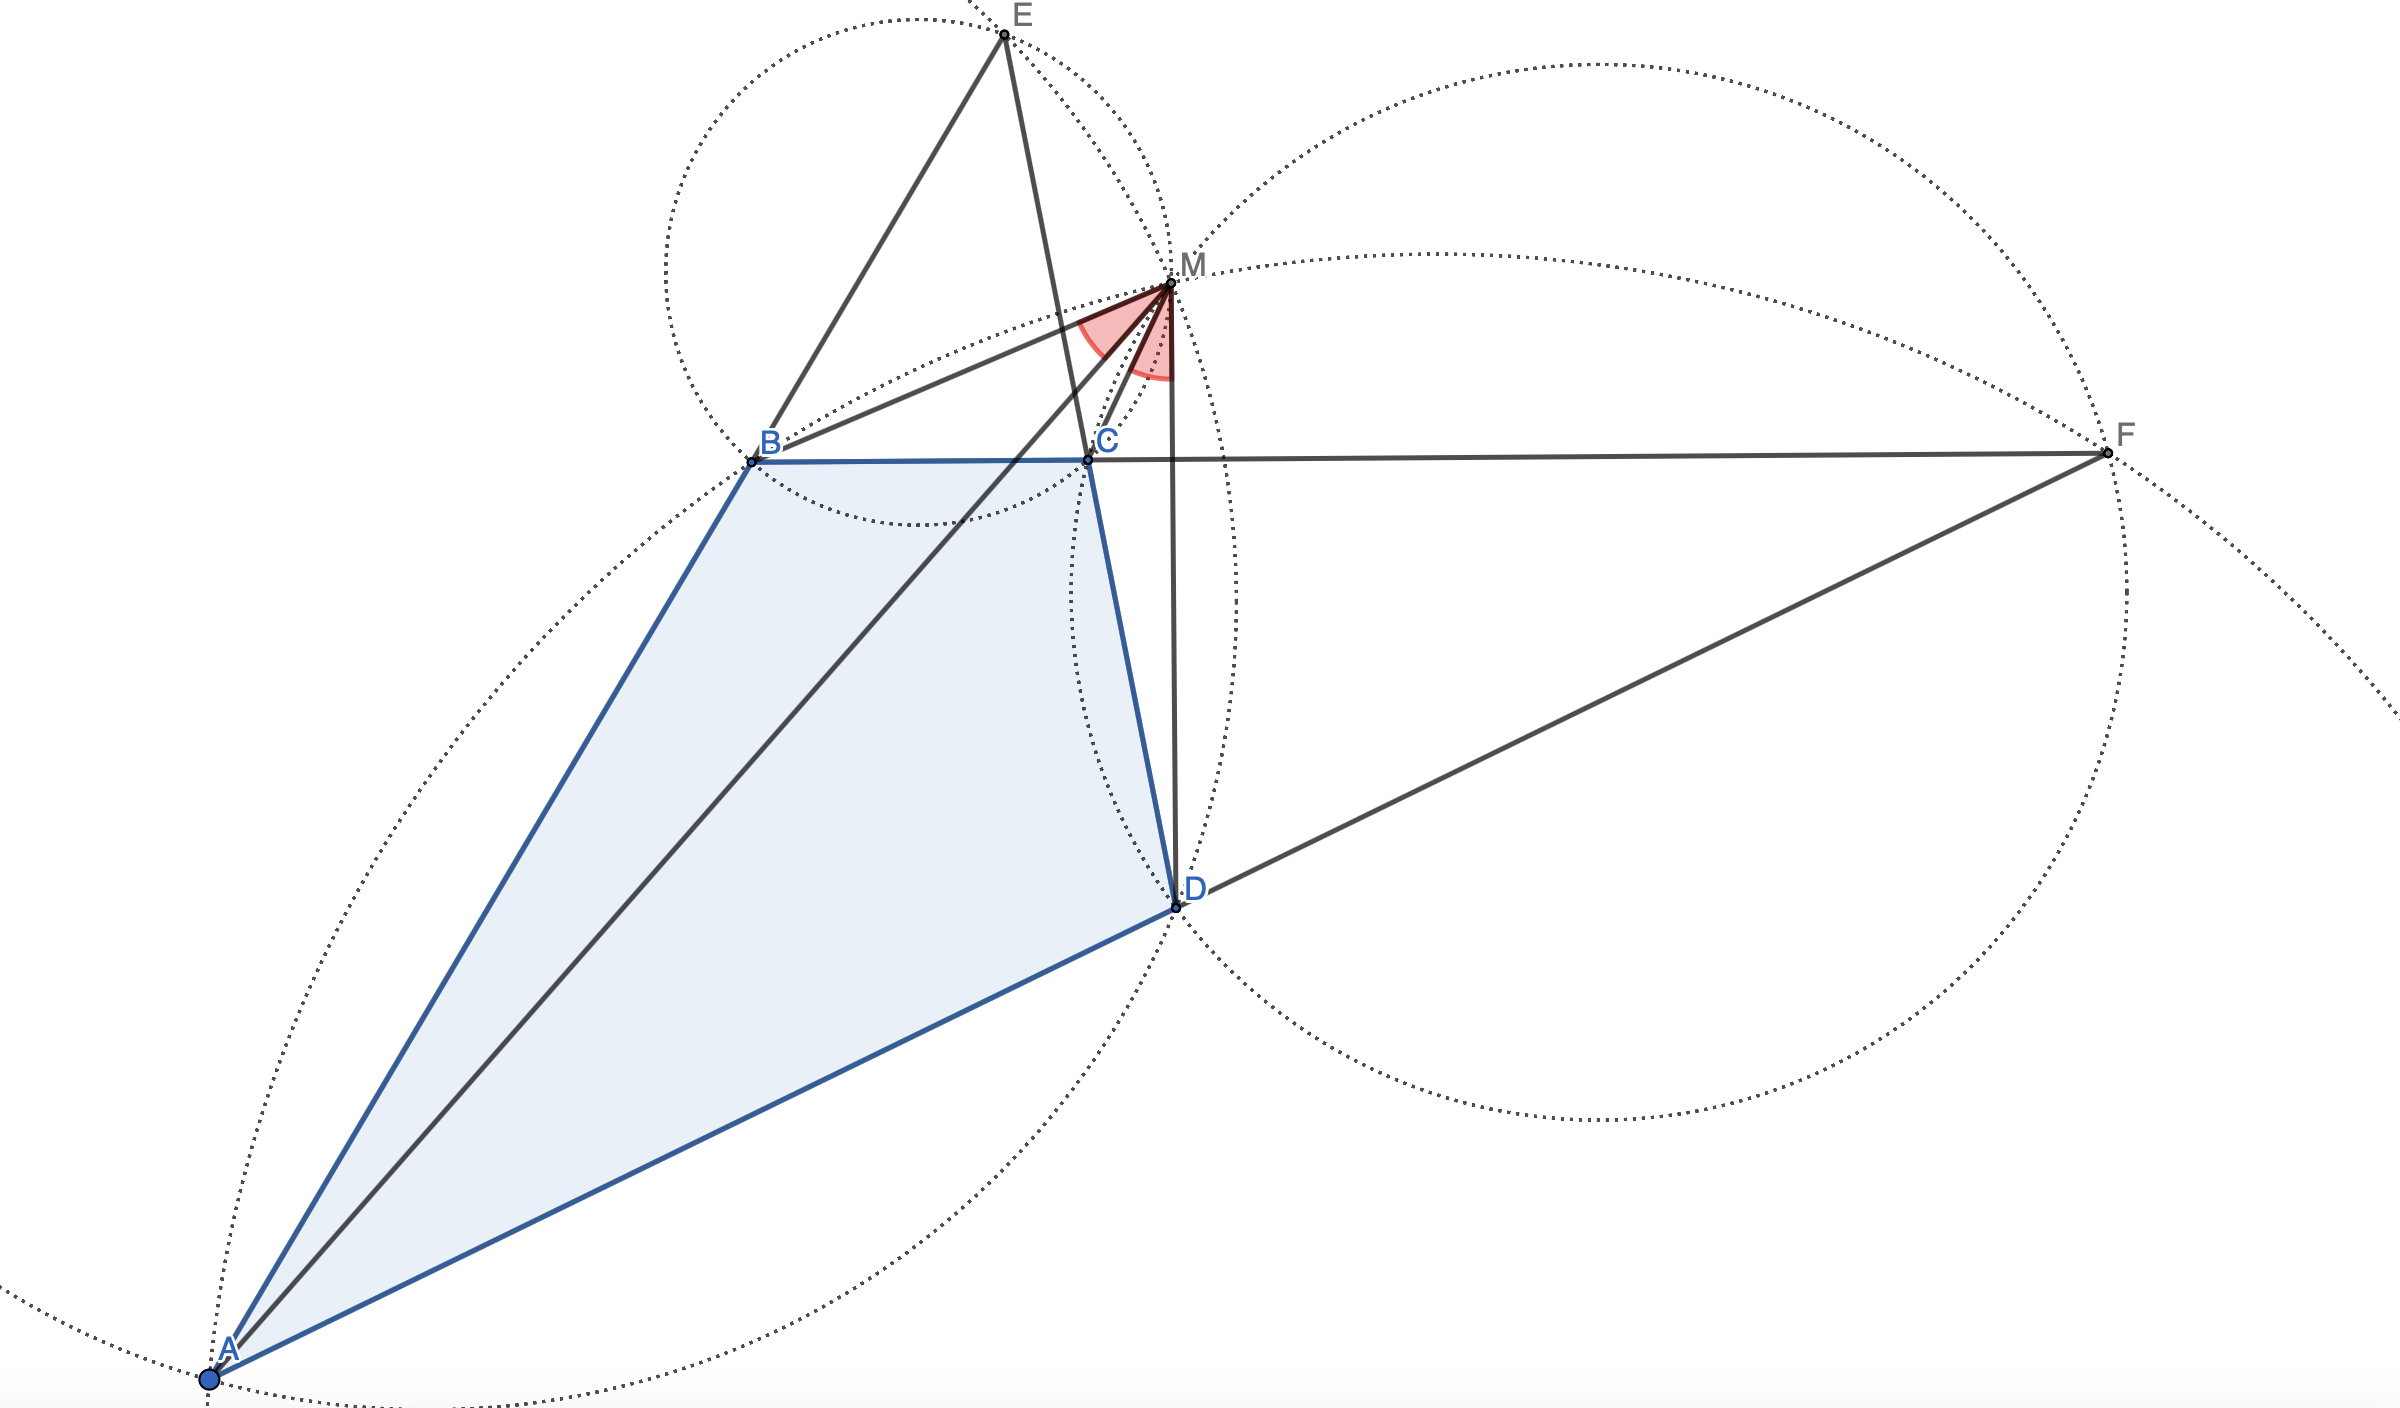
\includegraphics[width=1\textwidth]{Дабромат/II ступень/Решения/pics/Mikel's point.png}
\end{center}


(b) Докажите, что $M A \cdot M C=M B \cdot M D$.

\textbf{Решение.}
Треугольники $\vartriangle AMB$ и $\vartriangle DMC$ подобны, так как $\angle (MA, AB) = \angle (MA, AE) = \angle(MD, DE) = \angle (MD, DC)$. А из подобия и следует требуемое равенство.


\problem{2}
Четыре прямые общего положения высекают на плоскости четыре треугольника. Докажите, что центры описанных около этих треугольников окружностей лежат на одной окружности, проходящей через точку Микеля этих прямых.

\textbf{Решение.}

Покажем, что любая четверка точек из $O_1, O_2, O_3,O_4, M$ (см. рис.) лежат на одной окружности и тогда все пять будут лежать на одной окружности. Не умаляя общности будем доказывать, что $O_1, O_2, O_3, M$ лежат на одной окружности. 

\begin{center}
    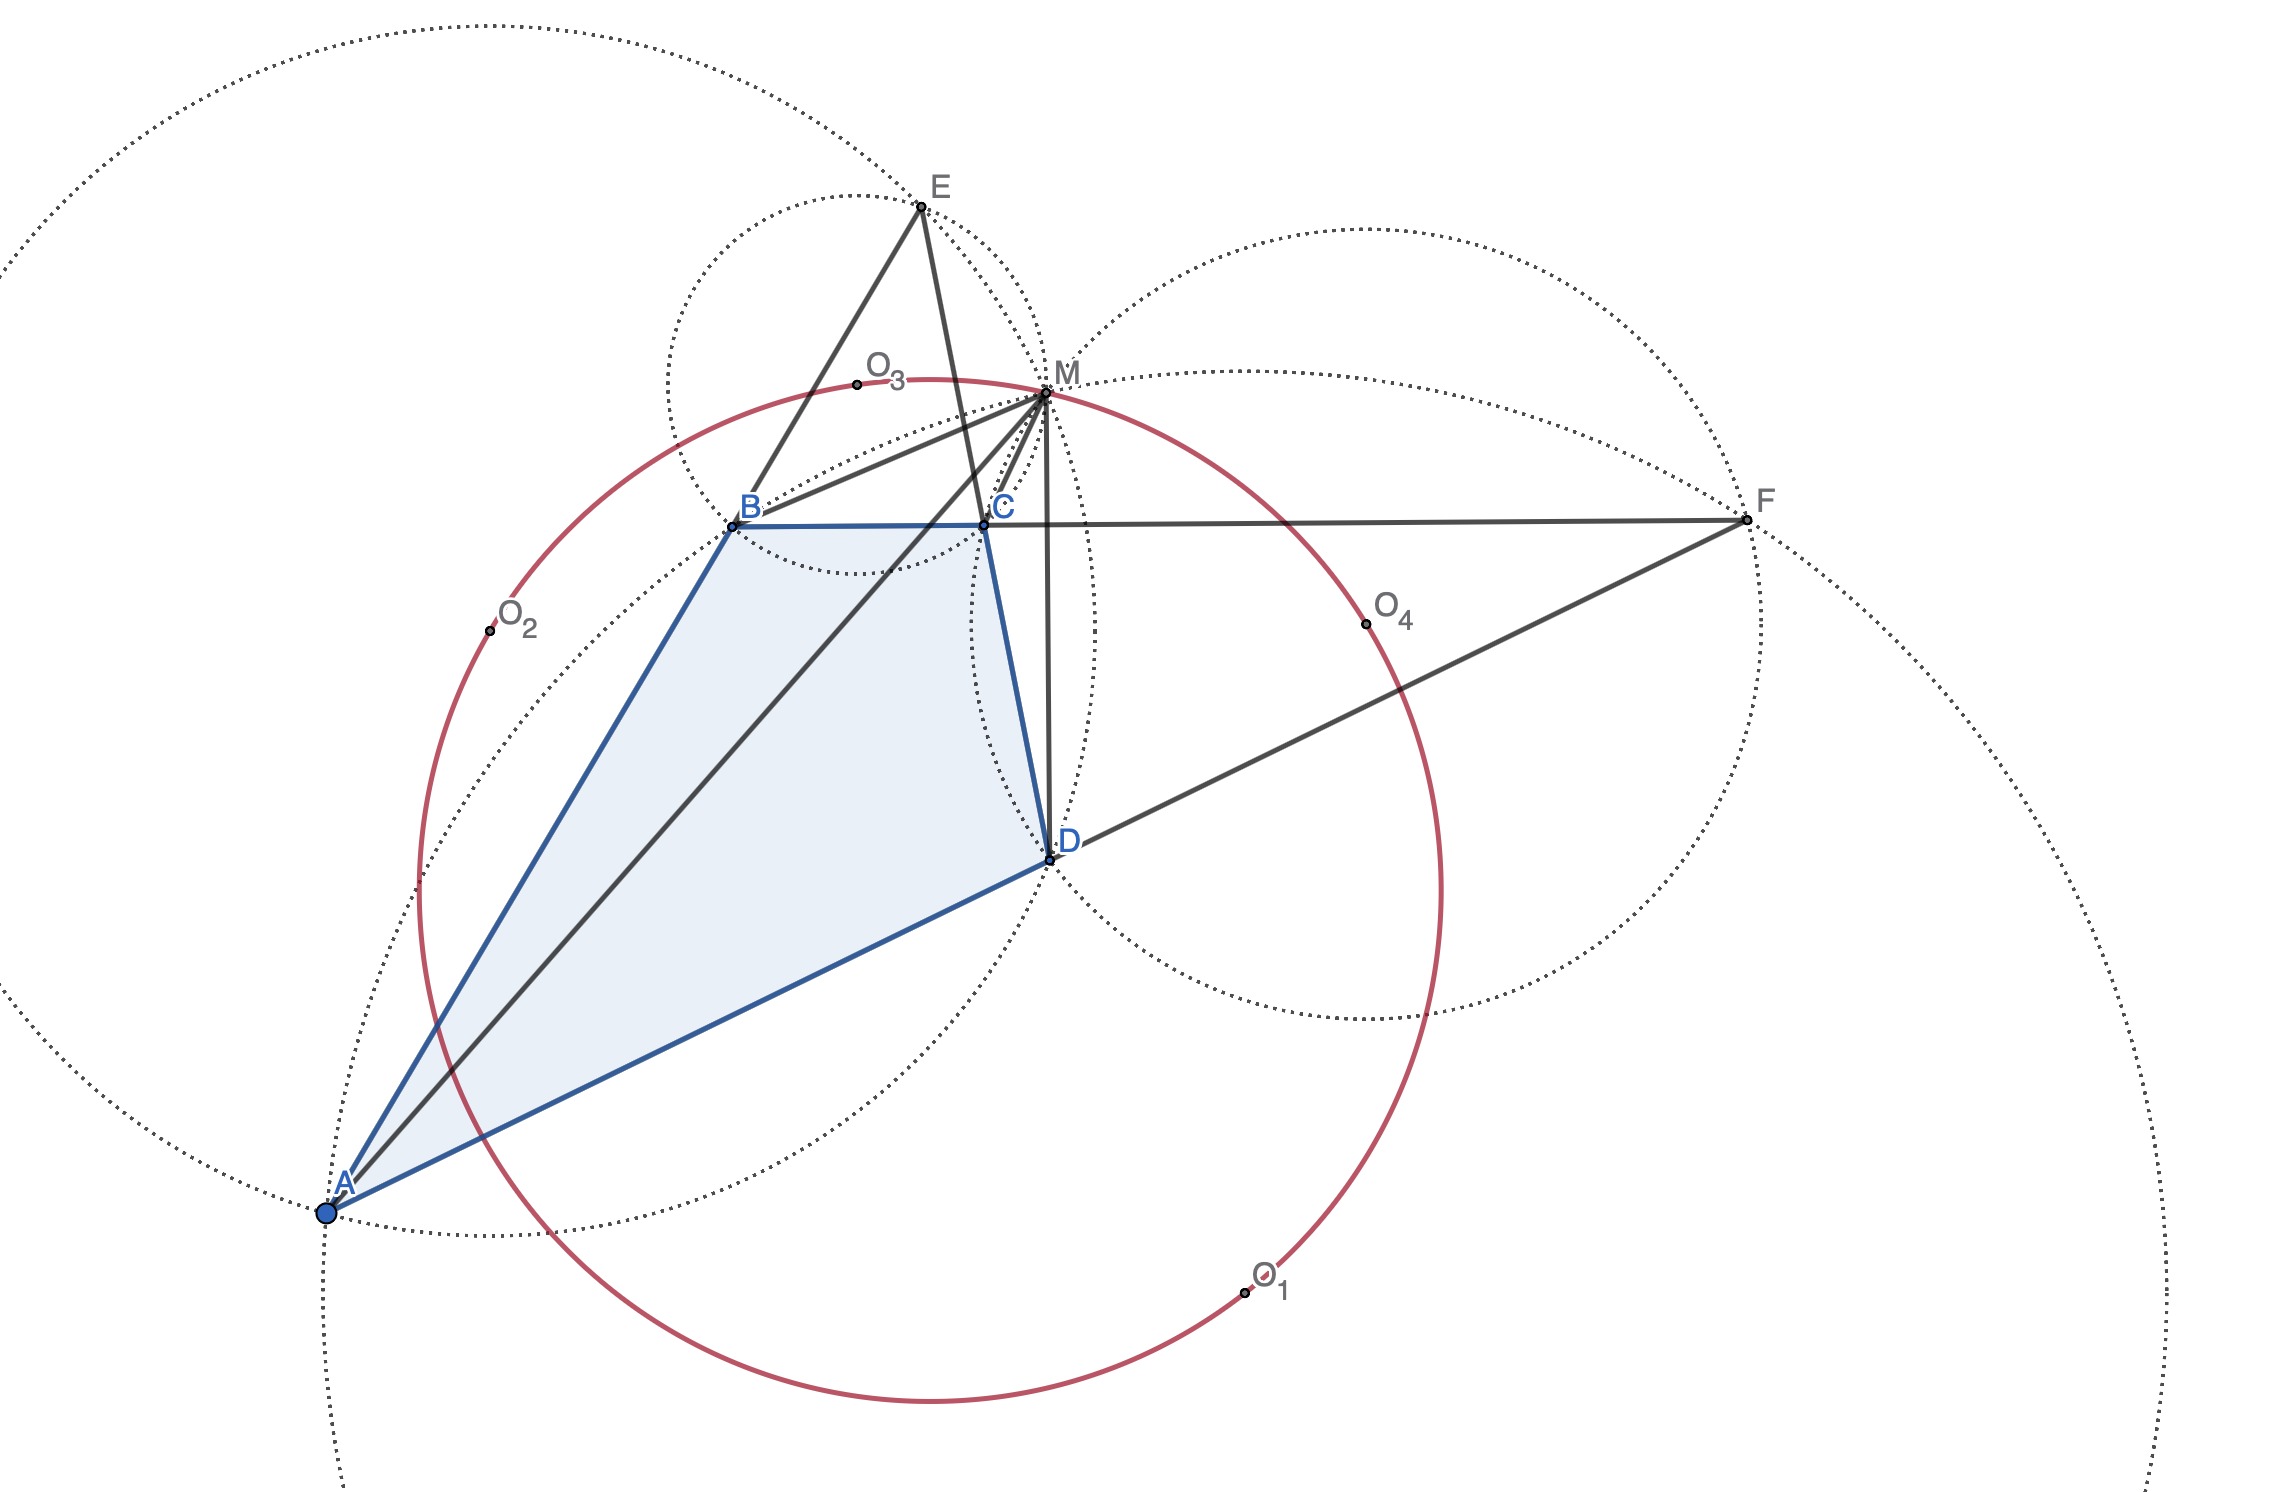
\includegraphics[width=1\textwidth]{Дабромат/II ступень/Решения/pics/Mikel's point_2.png}
\end{center}

\problem{3}
У четырехугольника $A B C D$ нет параллельных сторон. Прямая $\ell$ пересекает прямые, содержащие стороны четырехугольника, в четырех точках. Восстановим в каждой из этих точек перпендикуляр к соответствующей стороне четырехугольника. Докажите, что прямую $\ell$ можно выбрать так, чтобы эти перпендикуляры пересеклись в одной точке.

\textbf{Решение.}
Точка Микеля лежит на четырёх описанных окружностях образовавшихся треугольников. Следовательно, по теореме Симсона, её проекции на любые три из четырёх прямых лежат на одной прямой. Следовательно, все четыре проекции лежат на одной прямой(прямые Симсона точки Микеля для четырёх треугольников совпали)

\problem{4}
\textbf{5-окружность Микеля.} Даны пять прямых общего положения. Рассмотрим все пять точек Микеля всевозможных четверок этих прямых. Докажите, что получившееся пять точек будут лежать на одной окружности или прямой.

\textbf{Решение.}
\textit{Лемма о шестой окружности.} Во вписанном в (первую) окружность четырёхугольнике $A B C D$ через четыре пары вершин $A$ и $B, B$ и $C, C$ и $D, D$ и $A$ провели по одной окружности (еще четыре окружности) так, что точки их попарного пересечения $A_1, B_1, C_1, D_1$ лежат внутри первой окружности. Тогда $A_1, B_1, C_1, D_1$ лежат на одной (шестой) окружности.

\problem{5}
Дан четырехугольник $A B C D$, вписанный в окружность $\omega$ с центром в точке $O$. Прямые $A B$ и $C D$ пересекаются в точке $P$, а прямые $B C$ и $A D$ - в точке $Q$, а прямые $A C$ и $B D-$ в точке $R$.

(a) Докажите, что точка Микеля $M$ четверки прямых, содержащих стороны четырехугольника, лежит на прямой $P Q$.

\textbf{Решение.}
$\angle(PM, MB) = \angle (PC, CB) = \angle(CD, CB) = \angle(AB, AD) = \angle(MB, MQ)$

(b) Докажите, что четырехугольники $M A O C$ и $B O D M$ - вписанные.

\textbf{Решение.}
$\angle (AM, MC) = \angle(AM, MB) + \angle(MB, MC) = \angle(AQ, QB) + \angle(BP, PC) = \angle(AB, BD) + \angle(BD, BC) + \angle (AB, BD) + \angle(BD, CD) = \angle (AD, CD) + \angle(AB, BC) = 2 \angle (AD, DC) = \angle (AO, OC)$, что и требовалось доказать. Аналогично с другим четырехугольником.

(c) Докажите, что $M O \perp P Q$.

\textbf{Решение.}

    
(d) Покажите, что точка $R$ лежит на прямой $OM$ и выведите из этого, что $O R \perp P Q$.

\textbf{Решение.}
Из пункта $b$ мы знаем, что $MAOC$, $BODM$ вписанные. Рассмотрим окружности $(MAOC), (BODM), (ABCD).$ Прямая $AC$, являющаяся радикальной осью для окружностей $(ABCD)$ и $(MAOC)$ и прямая $CD$ являющаяся радикальной осью для окружностей $(ABCD)$ и $(BODM)$ пересекаются в точке $R$. Стало быть прямая $MO$, являющаяся радикальной осью для окружностей $(MAOC)$ и $(BODM)$ проходит через точку $R$. А так как $MO \perp PQ$ из предыдущего пункта, то и $OR \perp PQ$

(e) Теорема. Точка $O$ является ортоцентром треугольника $P Q R$

\textbf{Решение.}


(f) Обозначим за $X$ и $Y$ основания касательных, проведенных из точки $P$ к $\omega$. Докажите, что прямая $X Y$ проходит через точку $Q$.

\textbf{Решение.}

На сторонах $A B$ и $A C$ треугольника $A B C$ выбираются такие точки $P$ и $Q$, что четырехугольник $B P Q C$ вписан в окружность с центром в точке $O$. Диагонали четырехугольника пересекаются в точке $S$. Докажите, что прямая $O S$ проходит через одну из общих точек окружностей ($B A C$) и $(P A Q)$.